\section{Kilka słów o gramatykach}
Głównym celem pracy jest opracowanie gramatyki kształtu twarzy ludzkiej,
powinniśmy więc na samym początku dowiedzieć się czym właściwie jest ta
gramatyka kształtu.

Gramatyka jest ,,działem językoznawstwa zajmujący się badaniem reguł, które
rządzą generowaniem wyrazów i zdań języka''~\cite{wiki01}. Jak widać definicja
ta jest ściśle związana z lingwistyką, ale interesujące w tej definicji jest ,,badanie reguł'' oraz ,,generowanie wyrazów i zdań''.
Jeżeli tymi wyrazami są jakieś figury geometryczne (kształty) 2D bądź 3D:

\begin{figure}[h!]
\centering
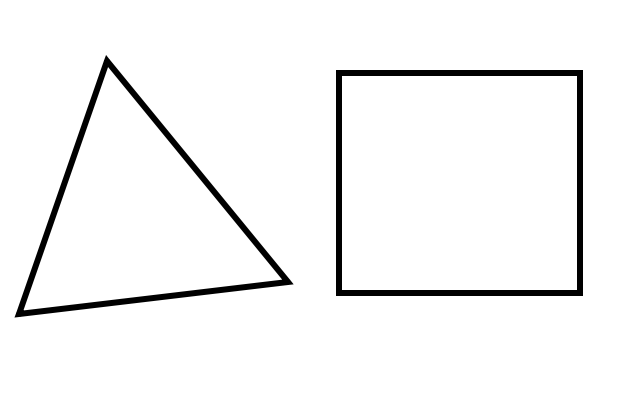
\includegraphics[width=6cm]{images/ksztalt.png}
\caption{Przykład podstawowych kształtów (źródło własne)}
\end{figure}
to regułami będą przekształcenia tych figur takie jak np. obrót, przesunięcie.

\begin{figure}[h!]
\centering
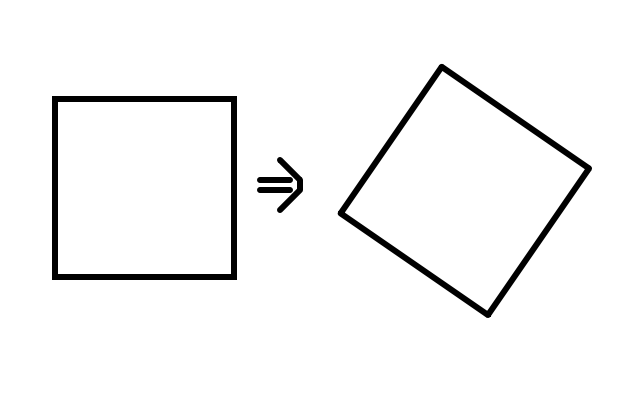
\includegraphics[width=6cm]{images/obrot.png}
\caption{Obrót kształtu (źródło własne)}
\end{figure}

Tak jak w językach wyrazy, tak i tu kształty mogą być dowolne, nawet bardzo
skomplikowane.
To skoro podstawowe kształty mogą być dowolnie skomplikowane to po co ta cała
gramatyka? Odpowiedź jest prosta - po co wymyślać wyrazy w języku, które
określają coś skomplikowanego jeśli można to opisać {\em zdaniem}. Czym w takim
razie jest zdanie? Jest to nic innego jak zbiór wyrazów połączonych
odpowiednimi regułami. I właśnie dzięki tym regułom możemy tworzyć
skomplikowane kształty.

W dalszej części rozdziału zostaną matematycznie przedstawione podstawowe
gramatyki wykorzystywane w grafice komputerowej (źródło~\cite{gaudi}). Jako
wprowadzenie do gramatyk kształtu można wykorzystać przykład prostej gramatyki, za pomocą
której możemy wygenerować strukturę butelki coca coli~\cite{link10}. Bazując na
zdjęciach różnych modeli butelki~\ref{coca_cola} można łatwo określić jej
logiczną budowę oraz utworzyć odpowiedni parametryczny kształt.

\addtocounter{footnote}{1}
\begin{figure}[h!]
\centering
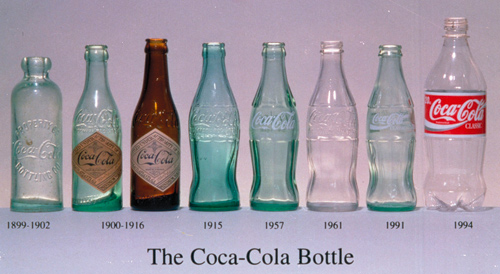
\includegraphics[width=14cm]{images/Coca-Cola.jpg}
\caption[Wybrane butelki napoju Coca Cola na przestrzeni
lat.]{Wybrane butelki napoju Coca Cola na przestrzeni
lat~$^{\decimal{footnote}}$.}
\label{coca_cola}
\end{figure}
\footnotetext[\value{footnote}]{\url{http://www.redesign-day.com/design-icons-the-coca-cola-bottle/}}

\begin{figure}[h!]
\centering
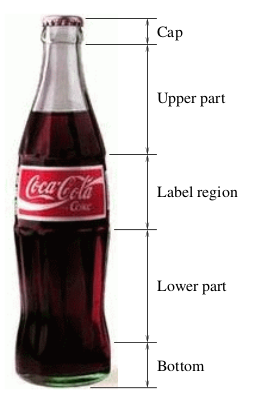
\includegraphics[width=5cm]{images/coca-cola_parts.png}
\caption{Podział butelki Coca Cola na logiczne części.~\cite{link10}}
\label{coca_cola_parts}
\end{figure}

Mając wydzielone logiczne części możemy rozpisać gramatykę kształtu zaczynając
od początkowego symbolu $*I$ poprzez kolejne $*U$ -- górna część, $*D$ -- dolna
część, $*T$ -- nakrętka.

\begin{figure}[h!]
\centering
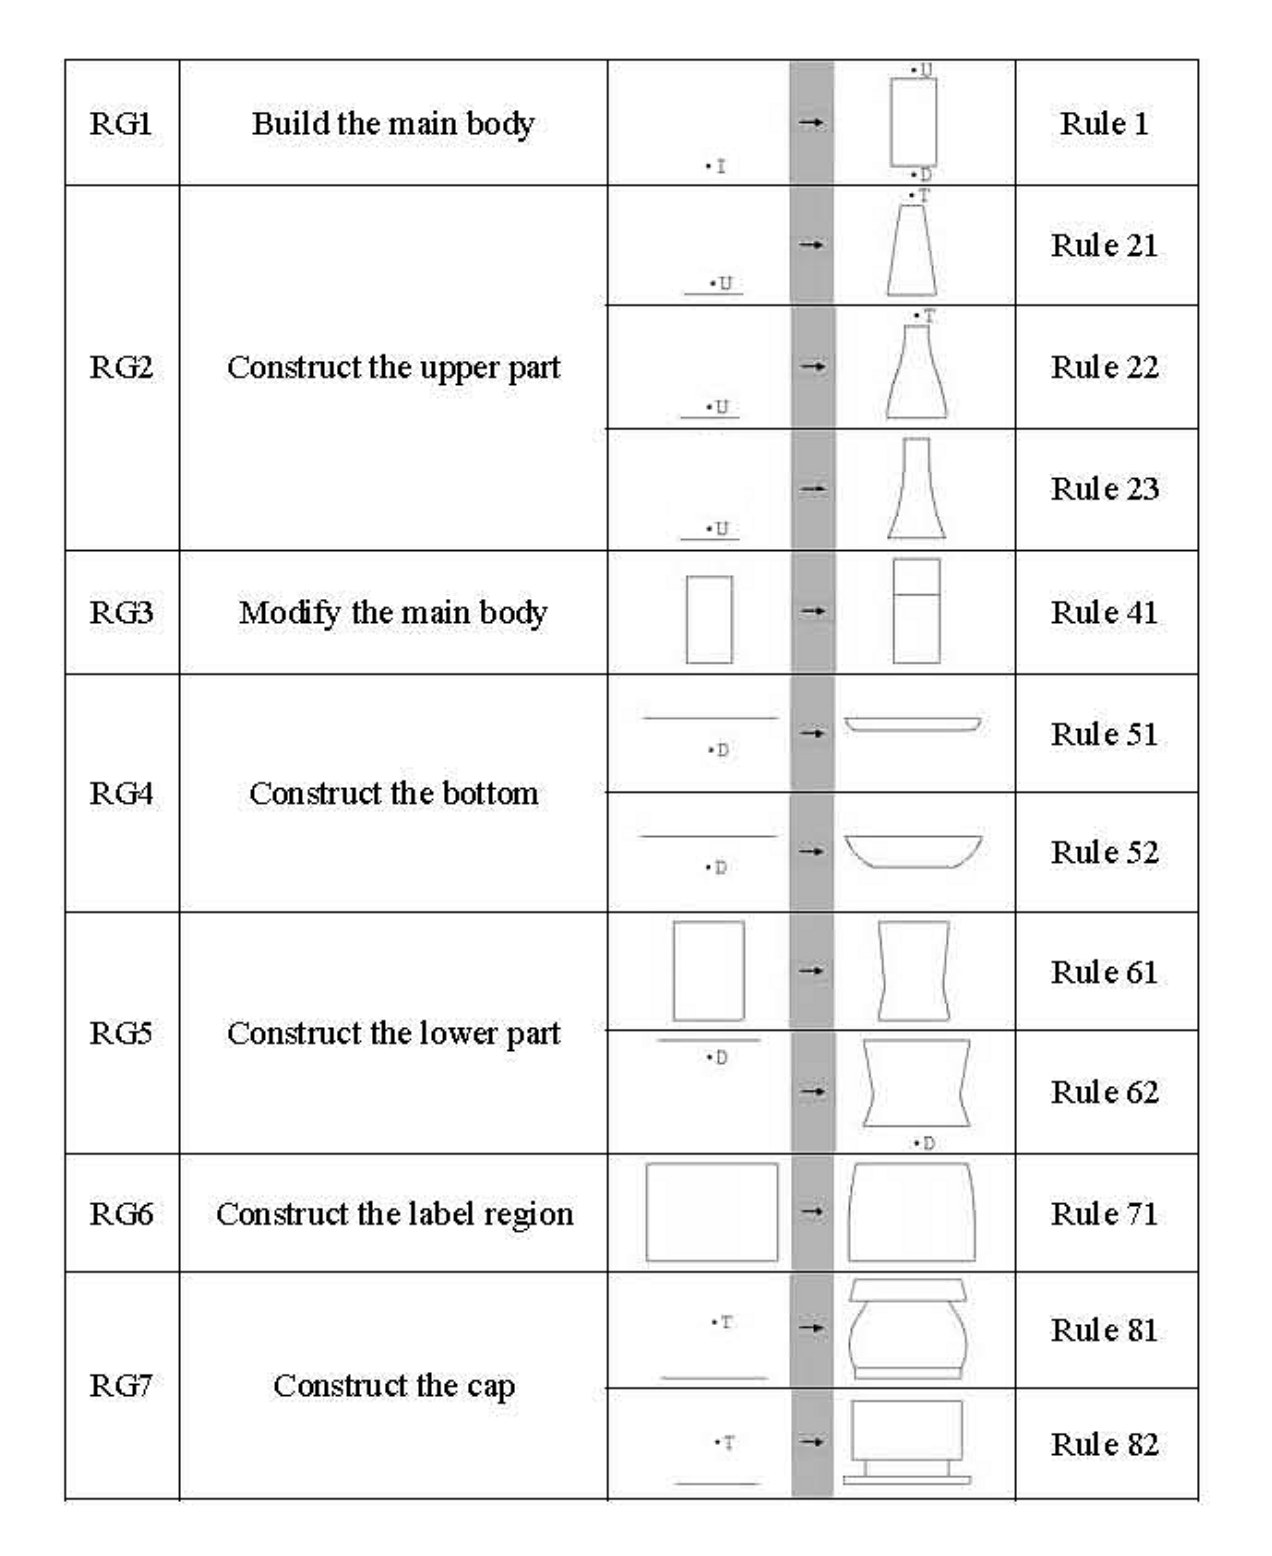
\includegraphics[width=12cm]{images/table01.png}
\caption{Reguły gramatyki kształtu do wygenerowania butelek
coca-coli.~\cite{link10}}
\label{coca-cola_regules}
\end{figure}

Przykład rozpisywania gramatyki od symbolu początkowego poprzez reguły aż do
uzyskania gotowych butelek znajduje się na ilustracji~\ref{coca_cola_create},
oraz wygenerowane wszystkie możliwe butelki z wykorzystaniem reguł
z~\ref{coca-cola_regules} znajduje się na ilustracji~\ref{coca_cola_all}.


\begin{figure}[h!]
\centering
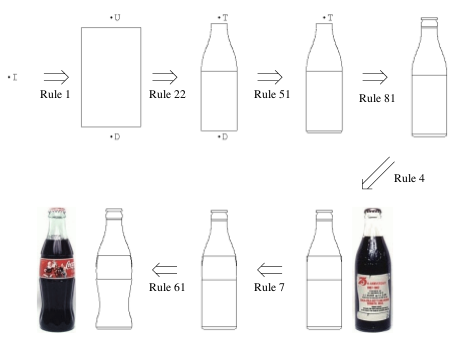
\includegraphics[width=9cm]{images/coca-cola_create.png}
\caption{Przykład generowania butelki na podstawie gramatyki
kształtu~\cite{link10}.}
\label{coca_cola_create}
\end{figure}

\begin{figure}[h!]
\centering
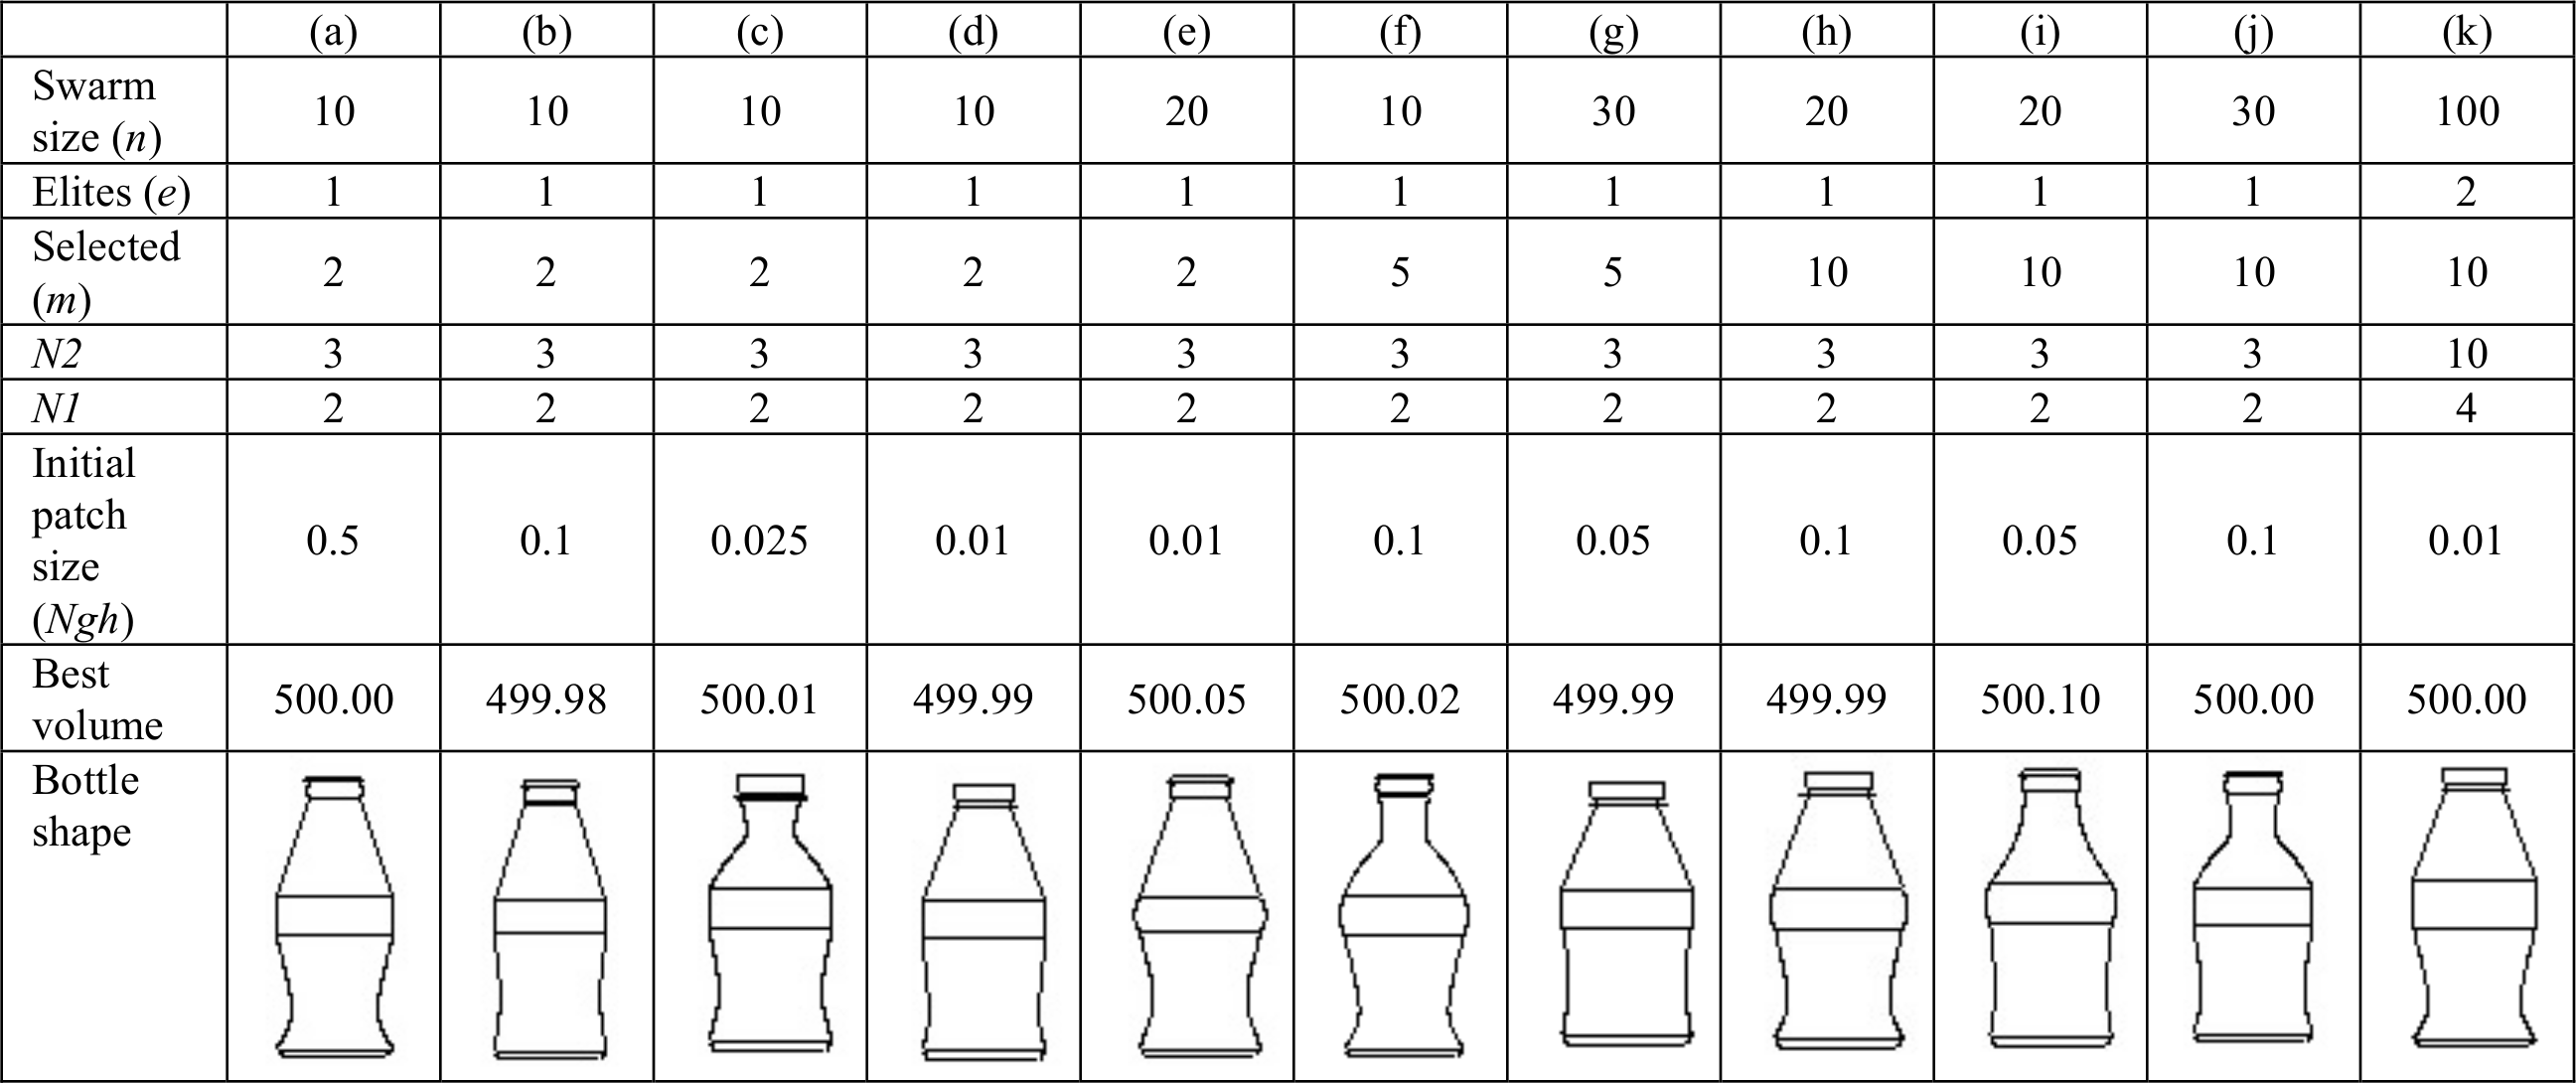
\includegraphics[width=15cm]{images/bootles.png}
\caption{Wygenerowane butelki na podstawie reguł~\cite{link10}}
\label{coca_cola_all}
\end{figure}

\subsection{Gramatyka formalna}
Gramatyka kształtu wywodzi się od gramatyki formalnej, dzięki której można
opisać skomplikowane struktury korzystając z podstawowych elementów.
Główną zaletą jest jej prostota i czytelność. Jest zatem doskonałym narzędziem
do grupowania elementów podobnych oraz ich generowania używając prostszych
części. W dalszej części zostaną matematycznie przedstawione gramatyki formalne.
Rozpocznijmy więc od definicji gramatyki formalnej -- ,,sposób opisu {\em języka
formalnego}, czyli podzbioru zbioru wszystkich słów skończonej długości nad
danym alfabetem''~\cite{wiki02}.

\subsubsection{Podstawowe pojęcia}
\begin{description}
 \item[Język formalny] podzbiór zbioru wszystkich {\em słów} nad pewnym {\em
alfabetem};
 \item[Alfabet] jest to niepusty, skończony zbiór symboli, np.:\\
$T1 = \{a, b, c,\ldots, x, y, z\}$ - alfabet łaciński;\\
$T2 = \{0,1\}$ - alfabet binarny;
 \item Niech $T$ będzie alfabetem, wtedy:\\
$T \neq \emptyset$, $\#T < \infty$\qquad ($\#T$ -- moc zbioru $T$);
 \item[Symbol] pojęcie nie definiowalne (synonimy: znak, litera);
 \item[Słowo] (synonim: łańcuch, wyraz) skończony ciąg zestawionych razem
symboli alfabetu;\\
Rekurencyjna definicja łańcucha nad alfabetem $T$:
  \begin{enumerate}
    \item jest łańcuchem nad $T$ ($\epsilon$ -- łańcuch pusty, niezawierający
    żadnego znaku);
    \item jeśli $x$ jest łańcuchem nad $T$ i $a \in T$ to $xa$ jest łańcuchem
    nad $T$;
    \item nic innego nie jest łańcuchem poza tym, co wynika z punktów (1) i (2).
  \end{enumerate}
 \item[Językiem] $L$ nad alfabetem $T$ nazywamy dowolny podzbiór $L$ zbioru
$T^*$, gdzie $T^*$ jest zbiorem wszystkich łańcuchów nad alfabetem $T$:
  \begin{equation}
  L \subseteq T^*
  \vspace{-10pt}
  \end{equation}
 \item Przykłady języków:
  \begin{description}
   \item[$L_0 = \emptyset$]-- język pusty;
   \item[$L_1 = \{\epsilon\}$]-- język zawierający tylko słowo puste;
   \item[$L_2 = T^*$]-- język zawierający wszystkie słowa nad alfabetem $T$;
   \item[$L_3 = \{\epsilon, 0, 01, 001\}$]-- język zawierający skończoną liczbę
  słów;
   \item[$L_4 = \{0, 01, 011, \ldots\} = \{01^n | n \ge 0\}$]-- język
  nieskończony.
  \end{description}
 \item[Gramatyka] $G$ nazywamy uporządkowaną czwórkę:
  \begin{equation}
  G = <N, T, P, Z>
  \vspace{-10pt}
  \end{equation}
 gdzie:
  \begin{description}
   \item[$N$]-- zbiór symboli nieterminalnych;
   \item[$T$]-- zbiór symboli terminalnych;
   \item[$P$]-- zbiór produkcji, z których każda ma postać
  $\alpha\rightarrow\beta$;
   \item[$Z\in N$]-- wyróżniony symbol początkowy (nieterminalny).
  \end{description}
 przy czym:
  \begin{description}
   \item[$P\subseteq (N\cup T)^+\times(N\cup T)^*$]
   \item[$P=\{\alpha\rightarrow\beta | \alpha\in(N\cup T)^+, \beta\in(N\cup
  T)^*\}$]
  \end{description}
 \item[Wyprowadzalność.] Słowo $\psi$ jest wyprowadzalne bezpośrednio ze słowa
$\omega$ w gramatyce G, co zapisujemy:
  \begin{equation}
  \omega \Longrightarrow_G \psi
  \vspace{-10pt}
  \end{equation}
jeśli:
  \begin{description}
   \item $\omega = \gamma\alpha\delta$;
   \item $\psi = \gamma\beta\delta$;
   \item $(\alpha\rightarrow\beta)\in P$;
   \item $\alpha,\beta,\gamma,\omega,\psi\in(N\cup T)^*$.
  \end{description}
Słowo $\psi$ jest wyprowadzane ze słowa $\omega$ w gramatyce $G$, co zapisujemy:
  \begin{description}
   \item $\omega \Longrightarrow_G^+\psi$
jeżeli istnieja $\varphi_0$, $\varphi_1$,\ldots,$\varphi_n\in(N\cup T)^*$
takie, że:
   \item $\varphi_0 = \omega$,
   \item $\varphi_n = \psi$,
   \item $\varphi_i-1 \Longleftrightarrow \varphi_i$,  $i = 1,2,\ldots,n$
  \end{description}
Sekwencje $\varphi_0$,$\varphi_1$,\ldots,$\varphi_n$ nazywamy wyprowadzeniem o
długości $n$.
Definiujemy ponad to:
  \begin{description}
   \item
$(\omega\Longrightarrow^*\psi)\Longleftrightarrow(\omega\Longrightarrow^+)\vee(\omega=\psi)$
  \end{description}
Relacje $\Longrightarrow^+$ oraz $\Longrightarrow^*$ są odpowiednio przechodnim
oraz przechodnim i zwrotnym domknięciem relacji bezpośredniej wyprowadzalności
$\Longrightarrow$. Jeżeli wiadomo, o jaką gramatykę chodzi, pomijamy dolny
indeks ,,G'' w oznaczeniu tych relacji pisząc po prostu: $\Longrightarrow^+$,
$\Longrightarrow^*$.
 \item[Jezyk.] Gramatyka jest jednym ze sposobów definiowania języka formalnego.
Mając daną gramatykę $G$ oznaczamy przez $L(G)$ zbiór wszystkich słów, które
mogą być w tej gramatyce wyprowadzone z symbolu początkowego $Z$. Zbiór ten
nazywamy językiem generowanym przez daną gramatykę:
  \begin{description}
   \item $L(G)={x\in T^*|Z\Longrightarrow^*x}$
  \end{description}
Aby zilustrować tą definicję, rozważmy gramatykę:
  \begin{description}
   \item $G=<N,T,P,S>$
  \end{description}
gdzie:
  \begin{description}
   \item $N={S,A,B}$
   \item $T={a,b,c}$
   \item $P={S\longrightarrow cAb, A\longrightarrow aBa, B\longrightarrow aBa,
B\longrightarrow cb}$
  \end{description}
Gramatyka ta generuje język $L(G)={ca^ncba^nb|n\geq 1}$
Dla przykładu: aby wygenerować słowo $caacbaab$ dla $n=2$ należy zastosować
nastepującą sekwencję produkcji:
  \begin{description}
   \item $S\longrightarrow cAb\longrightarrow caBab\longrightarrow
caaBaab\longrightarrow caacbaab$
  \end{description}
\end{description}
Noam Chomsky~\cite{chomsky} zdefiniował cztery klasy gramatyk oraz cztery klasy
języków formalnych:
 \begin{enumerate}
  \item gramatyki klasy 0 lub gramatyki nieograniczone (unrestricted). Produkcje
  w tego rodzaju gramatykach mają postać $\alpha\longrightarrow\beta$, gdzie
  $\alpha$ i $\beta$ są dowolnymi łańcuchami symboli tej gramatyki, przy czym
  $\alpha\neq\epsilon$. Nie nakłada żadnych ograniczeń na postać produkcji
  gramatyki w stosunku do ogólnej definicji gramatyki. Języki generowane przez
  gramatyki tego typu noszą nazwę {\em języków rekurencyjnie przeliczalnych};
  \item gramatyki klasy 1 lub gramatyki kontekstowe. Produkcje mają postać
  $\alpha\longrightarrow\beta$, gdzie $\alpha$ i $\beta$ są takimi łańcuchami
  tej gramatyki, ze łańcuch $\beta$ jest przynajmniej tak długi jak łańcuch
  $\alpha$ oraz dodatkowo dopuszczona jest produkcja $Z\longrightarrow\epsilon$,
  jeśli język zawiera słowo puste. Języki generowane przez tego typu gramatyki
  nazywane są {\em językami kontekstowymi};
  \item gramatyki klasy 2 lub gramatyki bezkontekstowe. Produkcje mają postać
  $A\longrightarrow\beta$, gdzie $A$ jest nieterminalem $(A\in N)$, zaś łańcuch
  $\beta$ jest dowolnym łańcuchem symboli tej gramatyki. Języki generowane przez
  tego typu gramatyki noszą nazwę {\em języków bezkontekstowych};
  \item gramatyki klasy 3 lub gramatyki regularne. Jeśli produkcje mają postać
  $A\longrightarrow xB$ lub $A\longrightarrow x$, gdzie $A$ i $B$ są
  nieterminalami $(A,B\in N)$, zaś łańcuch $x$ jest dowolnym łańcuchem symboli
  terminalnych tej gramatyki $(x\in T^*)$, to gramatykę taką nazywamy {\em
  gramatyką prawostronnie liniową}. Jeśli produkcje mają postać
  $A\longrightarrow Bx$ lub $A\longrightarrow x$, gdzie $A$ i $B$ są
  nieterminalami $(A,B\in N)$, zaś łańcuch $x$ jest dowolnym łańcuchem symboli
  terminalnych tej gramatyki $(x\in T^*)$, to gramatyki takie nazywamy {\em
  gramatykami lewostronnie liniowymi}.
\end{enumerate}
\subsection{Gramatyki stochastyczne}
Gramatyki stochastyczne są rozszerzeniem gramatyk łańcuchowych. Wprowadza się w
nich czynnik probabilistyczny. Oznacza to, że każda reguła jest powiązana z
pewnym prawdopodobieństwem, przy czym suma prawdopodobieństw wystąpienia reguł o
tych samych lewych stronach wynosi 1. Wybór produkcji do zastosowania w kolejnym
kroku procesu derywacji, realizowany jest poprzez losowanie z uwzględnieniem
czynnika prawdopodobieństwa, które może być zmieniane w całym procesie (na
przykład po wykonaniu reguły zmniejsza się jej czynnik).

Dla prostoty zapisu rozpatrzmy gramatyki bezkontekstowe. Analogicznie definicja
ta może być przedstawiona dla różnych klas gramatyk. Każda produkcja
$\alpha\longrightarrow\beta$ będzie miała postać $A\longrightarrow X_ij$, gdzie
$X_ij$ będzie łańcuchem stworzonym z nieterminali i terminali.
\\
Rozpatrzmy gramatykę:
\begin{equation}
G=<N,T,P,S>,
\vspace{-10pt}
\end{equation}
gdzie:
\begin{description}
\item $N={A_1, A_2, \ldots, A_m}$,
\item $A_1\longrightarrow X_{11}, A_2\longrightarrow X_{12}, \ldots,
A_n\longrightarrow X_{1n}, \ldots,$
\item $A_m\longrightarrow X_{m1}, A_m\longrightarrow X_{m2}, \ldots,
A_m\longrightarrow X_{mn}$, przy czym $X_{ij}\in (N\times T)^+$
\end{description}
Stochastyczną (bezkontekstową) gramatyką jest czwórka:
\begin{equation}
G_S=<N,T,P^S,S>
\vspace{-10pt}
\end{equation}
gdzie $N$, $T$ oraz $S$ są definiowane jak dla zwykłych gramatyk
bezkontekstowych, zaś $P^S$ jest zbiorem produkcji postaci
$(A_i\longrightarrow X_{ij},p_{ij})$, takim że $A_i\in N$, $X_{ij}\in (N\times
T)^+$ oraz $\displaystyle\sum_{j=0}^{n_i}p_{ij}=1$, dla $i=1,\ldots,m$, gdzie
$n_i$ oznacza liczbę produkcji, których lewa strona ma postać $A_i$.
Zapis dwóch produkcji o tych samych lewych stronach, ale o różnych
prawdopodobieństwach można przedstawić następująco:
\begin{enumerate}
  \item $S\longrightarrow AB : 0.3$
  \item $S\longrightarrow BA : 0.7$
\end{enumerate}
Taki zapis oznacza, że prawdopodobieństwo wykonania pierwszej produkcji jest
równe $0.3$, a drugiej produkcji $0.7$ w pojedynczym kroku przepisywania.
\subsection{Gramatyki wielowymiarowe}
Dotychczas opisane gramatyki dotyczyły wyłącznie jednowymiarowej przestrzeni,
gdzie jedyną relacją pomiędzy sąsiednimi symbolami w łańcuchu była konkatenacja.
Jeśli chodzi o zastosowanie tych gramatyk w grafice komputerowej, to jest ono
bardzo ograniczone, dlatego też stworzono na ich bazie gramatyki wielowymiarowe.
Poniżej zostaną opisane poszczególne rodzaje gramatyk wielowymiarowych.
\subsubsection{Gramatyki tablicowe}
Gramatyki tablicowe~\cite{chanda} są analogiczne do gramatyk łańcuchowych z
tym, że używane są do generowania bardziej skomplikowanych sekwencji symboli w dwu lub więcej
wymiarowej przestrzeni. Produkcje mają postać dwuwymiarowych wzorców osadzonych
na siatce zamiast liniowej sekwencji, jak to ma miejsce w jednowymiarowych
gramatykach. Cały łańcuch jest modelowany jako funkcja odwzorowywująca zbiór pól
na siatce w zbiór symboli terminalnych gramatyki oraz symbolu pustego (\#).
Pojęcie {\em łączności} dla tego typu łańcuchów jest zdefiniowane w oparciu o
współrzędne symbolu na siatce. Dwa punkty $(i,j)$ i $(h,k)$ są sąsiadami, czyli
są połączone jeśli $|i-h|+|j-k|=1$.
Tablica $\Sigma$ jest nazywana {\em złączoną}, jeśli dla wszystkich symboli
$A,B$ w tej tablicy, za wyjątkiem symboli pustych (\#), istnieje sekwencja
$A=A_0,A_1,A_2,\ldots,A_n=B$ symboli, różnych od symbolu pustego (ścieżka) taka,
że $A_i$ jest sąsiadem $A_{i-1}$. Definicja jasno określa, że wszystkie symbole
puste są ze sobą połączone. Nakłada się również pewne ograniczenia na to, w jaki
sposób definiowane są reguły. Mianowicie, reguły posiadają strukturę gramatyki
izometrycznej. Dla takiej gramatyki, dla każdej reguły
$\alpha\longrightarrow\beta$, długość $\alpha$ i $\beta$ musi być taka sama.
Przy takim ograniczeniu, generowany łańcuch zawsze będzie miał skończoną długość
(w początkowej konfiguracji), zatem także liczba możliwych łańcuchów będzie
skończona.

Jakkolwiek język gramatyki izomatrycznej $G$ jest zdefiniowany jako
zbiór terminalnych łańcuchów $\tau$, takich że nieskończony łańcuch
$\#^\infty\tau\#^\infty$ może być otrzymany w gramatyce $G$ z początkowego
łańcucha $\#^\infty S\#^\infty$. W związku z tym, włączając regułę zawierającą
znak ,,*'' otrzymujemy zmienną długość łańcucha.

W gramatykach tablicowych startujemy z nieskończoną dwuwymiarową tablicą
zawierającą symbole puste (\#) z początkowym symbolem na którejś z pozycji.
Każda reguła zastępuje jedną tablicę inną. Reguły powinny spełniać warunki
izometryczne w przeciwnym razie nie będzie jasne jak zamienić większą tablicę na
mniejszą i odwrotnie, utrzymując przy tym łączność.

Poniżej~\ref{g_tab} przedstawiony został przykładowy zbiór reguł gramatyki
tablicowej oraz wyprowadzienie przykładowego słowa.

\begin{figure}[h]
  \centering
  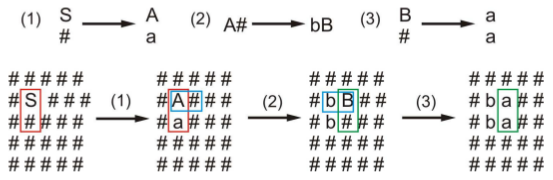
\includegraphics{images/g_tab.png}
  \caption{Proces generowania słowa w gramatykach tablicowych.~\cite{gaudi}}
  \label{g_tab}
\end{figure}

\subsubsection{Gramatyki grafowe.}
Łańcuchy oraz tablice mogą być rozpatrywane również jako specyficzne struktury
grafowe. Gramatyki grafowe są uogólnieniem gramatyk łańcuchowych na
grafy~\cite{chanda}. Liczba relacji pomiędzy sąsiadami może posiadać przypadkowe
wartości (zamiast 2 dla gramatyk łańcuchowych i 4 dla tablicowych). Proces tworzenia słowa za pomocą
gramatyki grafowej oparty jest o rozpoznawanie konkretnych podgrafów oraz ich
zastępowaniu zgodnie z produkcjami. Zatem, dla każdej reguły postaci
$\alpha\longrightarrow\beta$, $\alpha$ i $\beta$ powinny być reprezentowane
przez podgrafy i ich zamiana powinna polegać na tym, że $\alpha$ zostanie
usunięte z całego grafu i zastąpione przez $\beta$. Szczególnym przypadkiem
gramatyk tego rodzaju są gramatyki drzewiaste, których językiem (zbiorem
generowanych słów) jest zbiór struktur drzewiastych. Poniżej został
przedstawiony przykładowy zbiór reguł oraz przykładowy graf przez ten zbiór
wygenerowany~\ref{g_graf}.

\begin{figure}[h]
  \centering
  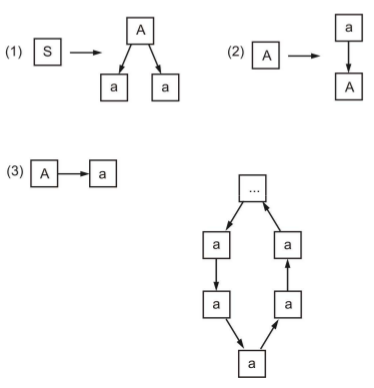
\includegraphics{images/g_graf.png}
  \caption{Przykład gramatyki grafowej, oraz wygenerowany przez nią
  graf.~\cite{gaudi}}
  \label{g_graf}
\end{figure}

\subsection{Gramatyki równoległe.}
Przedstawione wcześniej gramatyki wykorzystują model sekwencyjny zastępowania
symboli nieterminalnych. Jak wcześniej wspomniano mówimy, że gramatyka
$G=<N,T,P,S>$ akceptuje słowo $x$ jeśli istnieje ciąg takich produkcji:
\begin{equation}
X_0,X_1,\ldots,X_k:S\longrightarrow X_0\longrightarrow
X_1\longrightarrow\ldots\longrightarrow X_k=x,
\vspace{-10pt}
\end{equation}
gdzie każdy krok ($\longrightarrow$) oznacza zastąpienie tylko jednego elementu
prawej strony produkcji. W przypadku gramatyk równoległych, wprowadzono
dodatkowy warunek. Mówimy, że gramatyka równoległa (oznaczana dalej jako
$G^{||}$) akceptuje słowo $x$, jeśli istnieje taki ciąg równoległych produkcji
$X_0,X_1,\ldots,X_k:S\Longrightarrow X_0 \Longrightarrow
X_1\Longrightarrow\ldots\Longrightarrow X_k=x$ taki, że każdy krok iteracji
($\Longrightarrow$) oznacza wykonanie wszystkich możliwych zastąpień elementów
prawej strony. Efektem tego jest fakt, że języki akceptowane przez gramatyki
równoległe i równoważne im gramatyki sekwencyjne (wyłączając niektóre proste
przypadki) różnią się.
Rozważmy następujący przykład: mamy kolejne dwie produkcje: $S\longrightarrow
SS$, $S\longrightarrow a$, wtedy języki akceptowane przez te gramatyki wyglądają
następująco:
\begin{equation}
L(G)={a^n,n\geq 1}\\
L(G)={a^{2n},n\geq 1}
\vspace{-10pt}
\end{equation}
Tak więc w rzeczywistości język $L(G^{||})$ nie jest bezkontekstowy, mimo że
oparty jest na gramatyce bezkontekstowej. W przypadku gramatyk regularnych (po
prawej stronie produkcji występuje maksymalnie jeden terminal) języki przez nie
generowane są równoważne.

%% jakis kod

Gramatyki równoległe są wykorzystywane w grafice komputerowej przy realizacji
aplikacji opartych na systemach Lindenmeyera~\cite{lindenmeyer}. Te zostaną
omówione w kolejnej części rozdziału. Zalety stosowania tego podejścia są wielorakie: równoległość
daje, w przypadku dużych gramatyk możliwość rozproszenia aplikacji, przez co
uzyskujemy wysoką skalowalność i wydajność systemu. Ponadto fakt realizacji
wszystkich występujących w produkcji nieterminali w taki sam sposób pozwala na
uzyskanie w prosty sposób regularności tworzonego słowa.

\subsection{L-systemy.}
L-systemy (systemy Lindenmeyera)~\cite{lindenmeyer} początkowo stworzone zostały
na potrzeby symulacji wzrostu roślin w grafice komputerowej. Znalazły również zastosowanie w
generowaniu fraktali. Są one szczególnym przypadkiem automatów gramatyki
równoległej. Produkcje, jak w gramatykach łańcuchowych, stosuje się iteracyjnie
z góry określoną ilość razy, począwszy od pewnego stanu początkowego, zaś zbiory
reguł są stosunkowo małe.

Szczególnym przypadkiem L-systemów są systemy D0L (deterministyczne i
bezkontekstowe L-systemy). Charakteryzują się tym, że dla każdego nieterminala
mamy tylko jedną regułę, którą możemy zastosować. W przypadku, gdy istnieje
więcej produkcji możliwych do zastosowania dla pojedynczego terminala, oraz dla
każdej z nich przypisane jest jakieś prawdopodobieństwo to taki L-system
nazywamy stochastycznym.

Najbardziej popularnym i jednym z najbardziej rozpowszechnionych i
rozpoznawalnych języków programowania korzystających m.in. z idei L-systemów
jest język Logo. Oparty jest on na idei żółwia, którego ruchy definiuje
programista za pomocą prostych rozkazów (podniesienie, opuszczenie pisaka,
przesunięcie o określoną odległość w przód czy w tył, obrót żółwia o określony
kąt) z możliwością ich agregacji w procedury.

W najprostszych L-systemach stosuje się trzy sposoby zapisu gramatyki:
literalny, graficzny i proceduralny. Alfabet zapisu literalnego~\ref{fractal01}
opiera się na dwóch symbolach nieterminalnych: ,,F'' -- ruch w przód kursora,
,,-'' -- podnieś pisak i ,,+'' -- opuść. Za pomocą tych trzech symboli
definiowany jest symbol początkowy oraz produkcje. Drugim zapisem jest zapis
graficzny~\ref{fractal02}. Składa się on z dwóch części: symbolu początkowego
(inicjatora) oraz reguły (generatora), a sam proces generowania słowa przebiega
analogicznie jak w przypadku zapisu literalnego. Trzeci rodzaj zapisu jest zapis
proceduralny, realizowany np. przez wcześniej wspomniany język Logo.

L-systemy, w których stosuje się interpretacje żółwia umożliwiają tworzenie
bardzo zróżnicowanych obiektów, w tym przede wszystkim fraktale. Fraktale
charakteryzują się wysokim stopniem podobieństwa niezależnie od stopnia
złożoności, skali oraz fragmentu fraktala, który się obserwuje. Wraz ze wzrostem
(ilością wykonywanych iteracji) otrzymuje się ciekawsze kształty. Są proste do
tworzenia, ponieważ wymagają stosunkowo małego zbioru reguł (zwykle 1,2), a dają
bardzo dobre efekty graficzne. Większość z nich opiera się na zapisie
łańcuchowym, a symbole tworzące ostatni łańcuch interpretowane są np.: na ruchy
kursora (zgodnie z gramatyką żółwia). Przykładem takiego fraktala są np.: krzywa
Kocha, lub płatek śniegu. Proces budowy fraktali rozpoczyna się zazwyczaj od
prostego kształtu inicjującego, który w zapisie graficznym reprezentuje np.:
odcinek bądź łamaną, oraz jednej lub dwóch reguł, które są stosowane do każdego
symbolu w już wygenerowanym łańcuchu.

\addtocounter{footnote}{1}
\begin{figure}[h!]
  \centering
  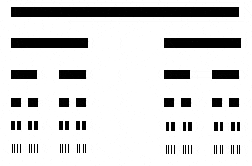
\includegraphics{images/fractal.png}
  \caption[Zbiór Cantora. F -- symbol początkowy, F-F+F --
  generator]{Zbiór Cantora. F -- symbol początkowy, F-F+F --
  generator~$^{\decimal{footnote}}$.}
  \label{fractal01}
\end{figure}
\footnotetext[\value{footnote}]{\url{http://pl.wikipedia.org/wiki/Zbi\%C3\%B3r\_Cantora}}
\addtocounter{footnote}{1}
\begin{figure}[h!]
  \centering
  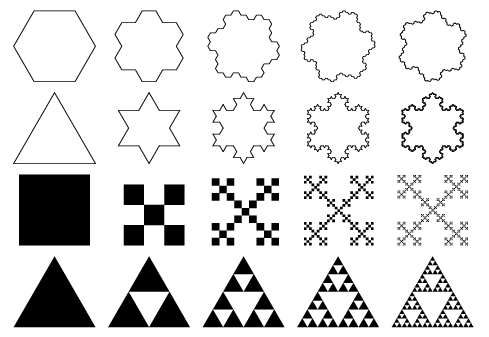
\includegraphics[width=11cm]{images/fractals.png}
  \caption[Inne przykłady fraktali]{Inne przykłady
  fraktali~$^{\decimal{footnote}}$.}
  \label{fractal02}
\end{figure}
\footnotetext[\value{footnote}]{\url{https://picasaweb.google.com/110433414991788678333/Fractals?fgl=true&pli=1}}

Początkowo działanie L-systemów w grafice było ograniczone do przestrzeni
dwuwymiarowych, jednak z czasem rozszerzono tą ideę do przestrzeni
trójwymiarowych (wprowadzono m.in. symbole rotacji względem dwóch pozostałych
osi).

Prusinkiewicz i Lindenmeyer w swojej pracy pod tytułem ,,The Algorithmic Beauty
of Plants''~\cite{abop} przedstawili możliwości wykorzystania L-systemów w
generowaniu modeli roślin (krzewów, drzew, kwiatów). Poszerzyli oni
funkcjonalność istniejącego systemu głównie poprzez dodanie trzeciego wymiaru,
sparametryzowanie gramatyki oraz dodanie tzw. procesu rozgałęziania poprzez
zastosowanie stosu do przechowywania aktualnego stanu kursora (pozycji,
kierunku, koloru oraz grubości rysowanej linii). Modyfikacje te pozwoliły
odwzorować naturalny dla świata roślin proces wzrostu.

Na ilustracji~\ref{fractal03} przedstawiony został przykład efektu rozgałęzienia
dla gramatyk dwuwymiarowych. W notacji literalnej takiego systemu odłożenie
aktualnego stanu kursora na stos używa się nawiasów kwadratowych.

\begin{figure}[h!]
  \centering
  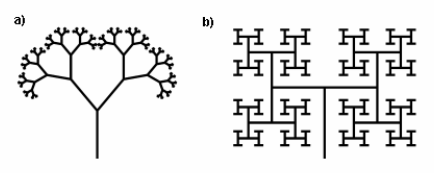
\includegraphics{images/fractal03.png}
  \caption{Fraktal drzewo dla kątów a) 30$^o$, b) 90$^o$.\cite{gaudi}}
  \label{fractal03}
\end{figure}

Zastosowania L-systemów są różnorakie, od tworzenia prostych kształtów
dwuwymiarowych i fraktali, poprzez generowanie trójwymiarowych obiektów i tworów
botanicznych, po tworzenie form graficznych na podstawie muzyki.

\begin{figure}[h!]
  \centering
  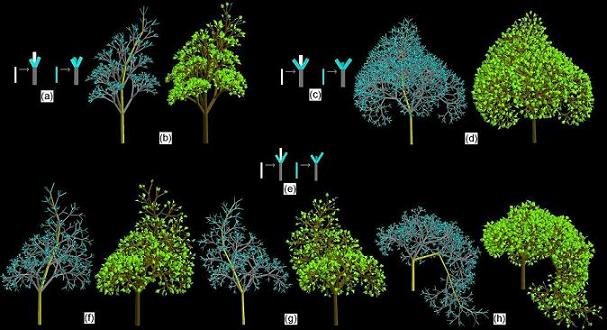
\includegraphics[width=12cm]{images/l-system01.jpg}
  \caption{Produkcje oraz wygenerowane za ich pomocą drzewa~\cite{ls01}.}
  \label{l-system01}
\end{figure}

\begin{figure}[h!]
  \centering
  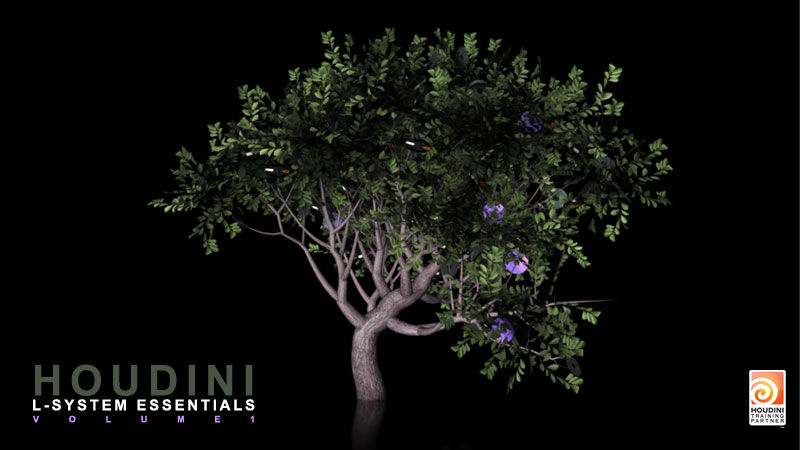
\includegraphics[width=10cm]{images/l-system02.jpg}
  \caption{Inny przykład wygenerowanego trójwymiarowego drzewa za pomocą
  L-systemów~\cite{ls02}.}
  \label{l-system02}
\end{figure}

\subsection{Gramatyki kształtu.}
Gramatyki kształtu zdefiniowane są jako czwórka $G=<S,L,P,I>$ gdzie $S$ jest
zbiorem kształtów, $L$ zbiorem symboli, $P$ zbiorem produkcji zaś $I$ jest
początkowym kształtem. Generowanie kształtu za pomocą tej gramatyki polega na
rozpoznaniu podkształtu, który ma być zastąpiony i jego zmianie na inny kształt
poprzez zastosowanie odpowiedniej produkcji. Dodatkowo w produkcjach, kształtom
można przypisać etykiety, które mogą determinować wybór kolejnej reguły oraz
sposób jej zastosowania.

\addtocounter{footnote}{1}
\begin{figure}[h!]
  \centering
  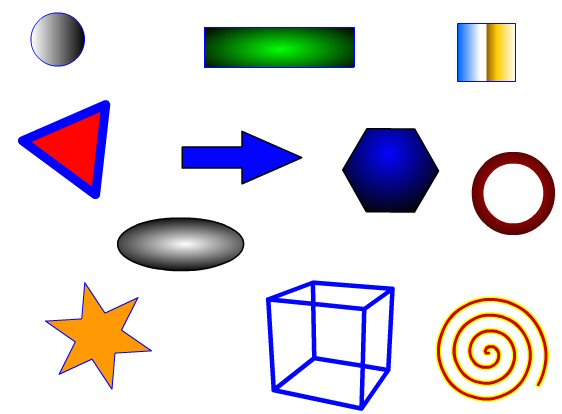
\includegraphics[width=11cm]{images/shapes.jpg}
  \caption[Przykłady różnych kształtów.]{Przykłady różnych
  kształtów~$^{\decimal{footnote}}$.}
  \label{shapes01}
\end{figure}
\footnotetext[\value{footnote}]{\url{http://www.parapal-online.co.uk/picture_dict/shapes.html}}


Dzięki zastosowaniu relacji przestrzennej między kształtami (przyleganie,
styczność, zawieranie, itp.), możliwe jest tworzenie innych bardziej złożonych
kształtów, np: opierając się na wiedzy na temat położenia dwóch figur, można
wykonać ich sumę, różnicę, lub inną operację, co daje większe zróżnicowanie
efektów. Dodatkowo, dobór produkcji do wykonania może być uwarunkowany
położeniem dwóch kształtów względem siebie.

%% rys str. 29

Do modyfikowania kształtów stosuje się proste operacje np.: przesunięcie,
rotacja, skalowanie i lustrzane odbicie względem prostej. Możliwe jest
zdefiniowanie większego zbioru operacji dodając nowe bądź poprzez połączenie już
istniejących transformacji w bardziej złożone.

\begin{figure}[h!]
  \centering
  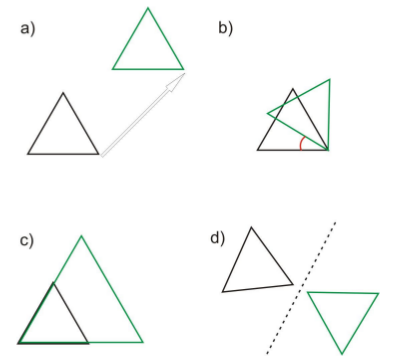
\includegraphics[width=8cm]{images/shapes02.png}
  \caption{Podstawowe transformacje w gramatykach kształtu a) przesunięcie, b)
  rotacja, c) skalowanie, d) lustrzane odbicie.\cite{gaudi}}
  \label{shapes02}
\end{figure}


Na ilustracji~\ref{etykietowanie} przedstawiony został przykład zastosowania
etykietowania kształtów. Etykieta determinuje tu sposób wykonania kolejnej produkcji. Dzięki
wprowadzeniu takiego rozwiązania można, za pomocą małego zbioru produkcji,
uzyskać bardziej złożone i zróżnicowane kształty. Możliwe jest wprowadzenie
kilku rodzajów etykietowania. Reguły mogą ponadto modyfikować istniejące
etykiety - zmienić ich położenie względem kształtu, usunąć etykietę, zastąpić
etykietę jednego rodzaju innym.

\begin{figure}[h!]
  \centering
  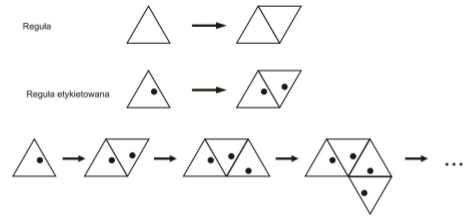
\includegraphics[width=12cm]{images/etykietowanie.png}
  \caption{Proces derywacji z zastosowaniem etykietowania.\cite{gaudi}}
  \label{etykietowanie}
\end{figure}

Gramatyki kształtu ze względu na swoje cechy stosowane są zazwyczaj do tworzenia
dwuwymiarowych obiektów, takich jak np.: posadzki, witraże, plany podstaw
budynków, ogrodów oraz plany zabudowy i plany pięter. Znajdują również
zastosowanie przy tworzeniu prostych, regularnych obiektów trójwymiarowych,
takich jak np. bryły budynków.

\subsection{Gramatyki --- podsumowanie.}
Ten rozdział miał na celu przedstawienie teorii dotyczącej gramatyk formalnych
skupiając się głównie na gramatykach stosowanych w grafice komputerowej.

W niniejszej pracy skupimy się na gramatykach kształtu oraz na gramatykach
grafowych (a raczej jej szczególnym rodzajem - gramatyki drzewiastej). Na
podstawie tych dwóch typów gramatyk spróbujemy opracować najwygodniejszą dla nas
gramatykę, za pomocą której postaramy się opisać głowę ludzką.
